%\documentclass[11pt]{article}

\documentclass[addpoints,10pt]{exam}

\usepackage[margin=2.5cm]{geometry}
\usepackage{graphicx}
\usepackage{listings}
\usepackage{xpatch}
\usepackage{color}
\usepackage{amsmath}

\makeatletter
\xpretocmd{\item@points@pageinfo}{\normalfont}{}{}
\xapptocmd{\item@points@pageinfo}{\bfseries}{}{}
\makeatother

\begin{document}
	\begin{center}
		\LARGE\scshape{Ley de Snell}
		
		\vspace{1cm}
		\large\scshape{Juan Barbosa - 201325901}
	\end{center}

	\begin{questions}
		{\question Calcular el \'indice de refracci\'on del material.}
				
		Usando la Ley de Snell:
		\begin{equation}
			n_i\sin(\theta_i) = n_r\sin(\theta_r)
		\end{equation}
		
		\begin{equation}
			\sin(\theta_i) = \dfrac{n_r}{n_i}\sin(\theta_r) \qquad y(x) = mx \qquad \text{donde $n_r = mn_i$}
		\end{equation}
		
		La incertidumbre en la pendiente se define como:
		
		\begin{equation}
			dm = \sqrt{\dfrac{\frac{1}{n-2}\sum\limits_{i = 1}^{n} \left(y_i - \hat{y}_i\right)^2} {\sum\limits_{i = 1}^{n}\left(x_i - \bar{x} \right)^2}}
		\end{equation}
		
		Teniendo en cuenta que $n_r = mn_i$, la incertidumbre en la pendiente da lugar a dos decimales, el \'indice de refracci\'on del aire difiere de 1, en la cuarta cifra decimal, por lo cual al nivel de precisi\'on experimental este se considera como 1.00. De esta forma:
		\begin{equation}
			n_r = 1.51
		\end{equation}
		\begin{figure}[h]
			\centering
			\includegraphics[width=0.6\linewidth]{indice.pdf}
		\end{figure}
		
		\newpage
		
		{\question Reflexi\'on interna total. Identificar los haces, encontrar el \'angulo cr\'itico.}
		
		La reflexi\'on interna total ocurre cuando el \'angulo de refracci\'on es mayor o igual a $\pi/2$.
		\begin{equation}
			n_r\sin(\theta_c) = n_i \qquad \longrightarrow \qquad \arcsin\left(\dfrac{n_i}{n_r}\right) = \theta_c \approx\arcsin\left(\dfrac{1}{n_r}\right) = 0.724\text{ rad} = 41.5^\circ
		\end{equation}
		
		El valor obtenido experimentalmente corresponde con $39^\circ$, lo cual representa un error de 6.02 \%. Es importante notar que en las fotograf\'ias se muestra que el rayo incidente entra en la direcci\'on radial, por lo cual en un sistema de coordenadas polares, este se hace coincidir con $\theta_0 = 0$. Si el valor del \'angulo incidente es 0, el rayo no es refractado y sigue una trayectoria recta.
		\begin{figure}[h]
			\centering
			\begin{tabular}{cc}
				\includegraphics[width=0.4\linewidth]{reflexionparcial.jpeg} &
				\includegraphics[width=0.4\linewidth]{reflexiontotal.jpeg} \\
				Reflexi\'on parcial & Reflexi\'on total
			\end{tabular}
		\end{figure}
		
		{\question Lente sencillo}
		
		En primer lugar se tomaron las distancias de la imagen al $3$ de la regla. Lo anterior da un ajuste de 4.6 cm al cero.
		
		\paragraph{$S_1 < f$:}
			Cuando se usan las leyes para lentes convergentes, es posible determinar que para esta regi\'on los rayos incidentes (izquierda) luego de pasar por el lente divergen, por lo cual no existe imagen. Sin embargo si se observa desde la parte derecha (derecha) es posible extrapolar los rayos hasta un punto donde convergen, en ese punto se forma la imagen virtual, que tiene mayor tama\~no que el objeto. El efecto anterior es el de una lupa.
			\begin{figure}[h]
				\centering
				\begin{tabular}{cc}
					\includegraphics[width = 0.4\linewidth]{lupa.jpeg} & \includegraphics[width = 0.4\linewidth]{bombillo.jpeg} \\
					Efecto lupa & Imagen projectada (filamento)
				\end{tabular}
				
			\end{figure}
			
		\paragraph{$f < S_1 < 2f$:} 
			Sobre este r\'egimen las im\'agenes se forman del lado derecho del lente, pero estas se encuentran invertidas. El aumento es mayor para $S_1 \approx f$ y va disminuyendo hasta el punto de no magnificaci\'on en $S_1 \approx 2f$. 
			\begin{figure}[h]
				\centering
				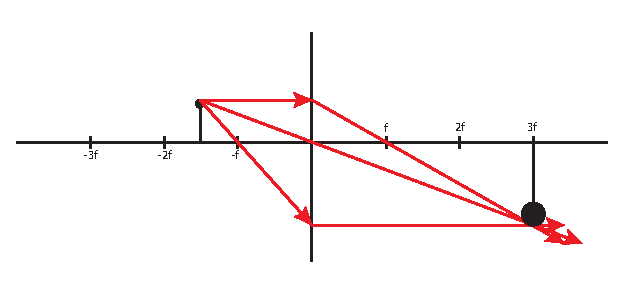
\includegraphics[width = 0.8\linewidth]{magnification.pdf}
			\end{figure}
			
			Para el caso de la imagen:
			\begin{equation}\label{1}
				\dfrac{1}{(3f/2)} + \dfrac{1}{S_i} = \dfrac{1}{f} \qquad \longrightarrow \qquad S_i = \dfrac{f(3f/2)}{(3f/2) - f} = 3f
			\end{equation}
			La magnitud es:
			\begin{equation}
				M = \dfrac{f}{f - S_o}
			\end{equation}
			
			Usando la ecuaci\'on (\ref{1}) es posible determinar $f$ en funci\'on de las distancias del objeto $(o)$ e imagen $(i)$.
			\begin{equation}
				f = \dfrac{S_iS_o}{S_i + S_o} \qquad \longrightarrow \qquad M = \dfrac{S_iS_o/(S_i + S_o)}{(S_iS_o/(S_i + S_o)) - S_o} = \dfrac{S_iS_o}{S_iS_o - S_iS_o - S_0^2} = -\dfrac{S_i}{S_o}
			\end{equation}
		
		\paragraph{$S_1 > 2f$:}
			La imagen se observa invertida y m\'as peque\~na.
			\begin{figure}[h]
				\centering
				\begin{tabular}{c}
					\includegraphics[width = 0.7\linewidth]{normal.jpeg} \\
					Imagen a 2f.
				\end{tabular}
				
			\end{figure}
			
		{\question Microsc\'opio b\'asico}
		El microsc\'opio constru\'ido es compuesto dado que tiene dos lentes. El objetivo, que es el primero en el camino \'optico magnifica poniendo el objeto en el r\'egimen de $f < S_1 < 2f$. El ocular es el segundo elemento \'optico, y tiene como objetivo hacer un efecto lupa sobre la imagen formada por el objetivo.
		
		La magnificaci\'on del objetivo es:
		\begin{equation}
			M_0 = \dfrac{f_0}{f_0 - s_0}
		\end{equation} 
		La magnificaci\'on del segundo es:
		\begin{equation}
			M_1 = \dfrac{f_1}{f_1 - s_1} \qquad \text{ donde $0<s_1<f_1$}
		\end{equation}
		
		La magnificaci\'on neta es:
		\begin{equation}
			M = M_0M_1 = \left(\dfrac{f_0}{f_0 - s_0}\right) \left(\dfrac{f_1}{f_1 - s_1}\right)
		\end{equation}
		
		De aca se observa que una misma magnificaci\'on $x$ puede ser conseguida independientemente del arreglo de lentes.
		
		Para medir la magnificaci\'on se project\'o la imagen sobre la pared, en donde determin\'o el tama\~no observado de la nariz en 3 cm, el cual media realmente cerca de 3 mm. Lo anterior representa un aumento de 10x. Sin embargo este ser\'ia mucho mayor si se considera el efecto lupa y se observa sobre el lente y no sobre la projecci\'on.
		
		
	\end{questions}
	
	
\end{document}
